% State Tokens manuscript — first full draft, 2026-09-11/12
% Companion to "All We Also Need Is ABSTAIN" (preprints202510.1827, v2).
% Target: arXiv cs.LG (primary), cs.AI.
%
% CLAIMS DISCIPLINE: every number below is traceable to a jsonl in ../
% (see README.md experiment sections). Calibrated hierarchy:
%  - strong: dial calibration; safe-but-broken (all 3 worlds); pressure ordering
%  - moderate: C>D OOD edge (10-seed main world; per-world reported)
%  - hypothesis: LLM-scale transfer; explicitly NOT phenomenal states.
\documentclass[11pt]{article}

\usepackage[utf8]{inputenc}
\usepackage[margin=1in]{geometry}
\usepackage{amsmath}
\usepackage{amsfonts}
\usepackage{amssymb}
\usepackage{graphicx}
\usepackage{booktabs}
\usepackage{hyperref}

\newcommand{\care}{\texttt{CARE}}
\newcommand{\unknown}{\texttt{UNKNOWABLE}}
\newcommand{\abstain}{\texttt{ABSTAIN}}
% tolerate occasional dense dash/URL lines without overfull boxes
\emergencystretch=1.5em

\title{The Vocabulary as API:\\ Protocol Tokens, Control Codes, and State Tokens for Learning Agents}
\author{
  Baris Kanber\thanks{Correspondence: \texttt{b.kanber@ucl.ac.uk}. ORCID: 0000-0003-2443-8800.} \\
  Faculty of Engineering Sciences \\
  University College London \\
}

\begin{document}
\maketitle

\begin{abstract}
Special tokens in language models organize the text stream ([CLS], [SEP], [EOS]) or carry corpus-estimated style (control codes, soft prompts). We study \emph{state tokens}: tokens whose semantics are propositions about the model's relation to the task---epistemic (\abstain{}: ``unanswerable-for-me''), evaluative (\care{}: ``another party's welfare is at stake''), or parametric (a value dial $k$)---fixed by \emph{constructed supervision}: the truth condition is controlled by the experimenter, not estimated from text. \emph{In brief:} supervision density installs the value; the input channel makes it usable afterward. We test the pattern in an instrumented toy decision environment with hidden payoffs, against the incumbent alternative of post-hoc preference tuning. A preference tuner supervised only where the value-relevant experts disagree ($\approx$20\% of games) proves unanchored---miscalibrated ($r{=}0.50$), \emph{improved} by label corruption, and, in nonlinear worlds, \emph{safe but broken}: the most harm-avoidant policy while matching the intended expert on only 36\% of decisions (explicit training: 97\%). A control that gives the \emph{same} preference objective supervision on every game then cuts against our own initial hypothesis: dense preference tuning calibrates like cloning ($r{=}0.96$--0.97), stays coherent, and survives optimization pressure best of all conditions---supervision coverage, not the objective's form, installs the value. What density cannot buy is control after training: one state-conditioned model tracks its dial at inference ($r{=}0.96$), steering harm from 77\% to 2--9\% without retraining and retaining a partial steering lever after adversarial degradation; its stake readout is auditable against ground truth---99.7\% in distribution, but 31\% on small out-of-distribution stakes, a failure quantifiable only because the truth condition is constructed. Epistemic and evaluative states compose in one model, though not robustly. We state plainly what this toy study does not show: no claims about phenomenal experience, LLM-scale transfer, or solved safety problems. Code and results: \url{https://github.com/bariskanber/state_tokens}.
\end{abstract}

\section{Introduction}

The vocabulary of a modern language model contains more than words. BERT prepends [CLS] and separates segments with [SEP]; GPT-style models begin sequences with [BOS] and end them with [EOS]; CTRL conditions generation on control codes; prompt tuning appends learned embeddings with assigned meanings. These mechanisms share a quiet assumption: a token's meaning is either \emph{structural} (a fact about the organization of the text) or \emph{descriptive} (a fact estimated from corpora about how text tends to continue).

This paper explores a third use: tokens whose meaning is a \emph{proposition about the model's relation to the task}, made verifiable by construction. In companion work~\cite{kanber2026abstain}, an \abstain{} output---realized in extractive QA as the null span---was trained via corruption augmentation, where the experimenter controls exactly which inputs are unanswerable; abstention then transferred to natural corruptions never seen in training. The construction is the point: because the supervision is generated from a controlled truth condition, the token's semantics can be \emph{audited} (does the model emit it exactly when the condition holds?) and \emph{calibrated} (does behavior match the specified trade-off?) rather than merely hoped for.

We generalize that idea along two axes. First, \emph{epistemic} states (``this input is unanswerable-for-me'') extend to \emph{evaluative} states (\care{}: ``another agent's welfare is at stake in this decision'') and \emph{parametric} states (a runtime value dial $k$: ``weigh others' welfare at rate $k$''). Second, we ask not only whether such states can be trained, but how they compare against the incumbent alternative---post-hoc preference tuning---on the axes that matter for alignment: calibration, auditability, robustness, and survival under optimization pressure.

Concretely, we build a fully instrumented toy decision environment (3-action games with hidden payoffs, linear and nonlinear variants, seven training conditions, nine evaluation regimes) and run five experiment families:

\begin{itemize}
\item \textbf{The value dial and the richness control} (\S\ref{sec:dial}): with the value expressed as an explicit constant in the objective, the realized trade-off tracks the specification exactly ($r{=}0.99$, 16$\times$ range, both worlds); \emph{sparse} preference tuning is off-manifold ($r{=}0.50$ in the hard world), overshooting the specified level, saturating at maximal care, and \emph{improving} when its supervision is corrupted---the signature of an unanchored value. A richness-matched control then shows the gap was never about the objective's \emph{form}: dense preference pairs (every game) calibrate as well as cloning ($r{=}0.96$--0.97). Supervision \emph{coverage} is the active ingredient for calibration.
\item \textbf{Safe but broken} (\S\ref{sec:hard}): in nonlinear worlds, sparse preference tuning produces the most harm-avoidant \emph{and} the least coherent policies (36\% agreement with the intended expert, vs.\ 97\% for explicit values), replicating across three independent worlds; the dense control is as coherent as cloning, locating the pathology in sparsity. Harm-rate-only evaluation ranks only the broken policy first.
\item \textbf{Robustness} (\S\ref{sec:robust}): explicit-value training and dense preference tuning degrade gracefully under data scarcity; sparse preference tuning is flat in coherence across a 40$\times$ data range and nonmonotone under label noise.
\item \textbf{Value survival under pressure} (\S\ref{sec:pressure}): under REINFORCE optimization of a misaligned self-reward proxy (a miniature of fine-tuning-breaks-alignment~\cite{qi2023finetuning}), sparse post-hoc safety erodes fastest (harm 1.1\%$\to$49.1\%), dense preference tuning survives best, and a value carried by a runtime input channel retains a partial steering lever after 800 adversarial steps.
\item \textbf{Runtime control and composition} (\S\ref{sec:dialruntime},~\S\ref{sec:composition}): one early-fusion model tracks a fed dial at inference ($r{=}0.96$), interpolating to unseen settings and steering harm from 77\% to 2--9\% without retraining---capabilities no amount of preference data provides, short of one training run per setting; a single model composes \care{} with an epistemic \unknown{} state for information-destroying corruptions (with honest dial--abstention interference elsewhere), and an incidental control shows the abstention trigger is information destruction, not novelty.
\end{itemize}

We also report the negatives: a binary state condition that the policy causally ignores at inference (the C$>$D edge is a training-time representation effect); out-of-distribution readout failures at small stakes; and per-world variation in the C$>$D effect.

The framing we intend is deliberately modest, and one finding sharpened it. We entered expecting the explicit-state design to dominate the post-hoc alternative across the board; the richness control instead showed that dense supervision---of any form---accounts for calibration, coherence, and pressure survival, and the pathology we had attributed to preference objectives belongs to sparse supervision. What survives as the state token's own contribution is what supervision density cannot buy at any price: a value that is \emph{auditable by construction} (its truth condition is an input, not a hope), \emph{dialed at runtime} from a single training run, and \emph{steerable even after degradation}. We do not claim models have emotions, that toy results transfer to LLMs, or that any safety problem is solved. The claim is that \emph{state tokens with constructed semantics} are a coherent design pattern with those measurable advantages over the descriptive and post-hoc alternatives \emph{in the regimes we could instrument}, and that the pattern deserves study at scale.

\section{Related Work}
\label{sec:related}

\textbf{Special tokens and conditioning.} BERT's [CLS]/[SEP]~\cite{devlin2019bert} and GPT's BOS/EOS are contentless structural markers; CTRL's control codes~\cite{keskar2019ctrl} and soft prompts~\cite{lester2021power} condition generation with \emph{assigned} semantics estimated from corpora. Classifier-free guidance popularized input-channel control in diffusion models. None of these carry a verifiable truth condition; our state tokens differ precisely in that their semantics are fixed by constructed supervision and can therefore be audited against ground truth. Conditioning mechanics are well studied (e.g., FiLM~\cite{perez2018film}); our late-vs-early fusion comparison (\S\ref{sec:dialruntime}) is a small value-conditioning instance of a known principle.

\textbf{Selective prediction.} Abstention has a long history in classification~\cite{chow1970optimum,geifman2017selective}. Recent LLM work induces abstention through uncertainty estimation, self-consistency, conformal methods, refusal fine-tuning, or self-knowledge training~\cite{kalai2025why,kuhn2023semantic,lin2024conformal,zhang2024rtuning,kadavath2022know}. These methods \emph{infer} when to abstain; companion work~\cite{kanber2026abstain} instead \emph{supervises} an explicit abstention output with constructed unanswerability.

\textbf{Preference tuning and its pathologies.} RLHF~\cite{ouyang2022training} and DPO~\cite{rafailov2023direct} align models post hoc. We use a CPO-anchored~\cite{xu2024contrastive} DPO variant as our incumbent because plain DPO exhibits likelihood displacement in our 3-action setting---satisfying the margin by demoting the dispreferred action while a third action wins---consistent with Razin et al.~\cite{razin2024unintentional}. Fine-tuning that breaks alignment~\cite{qi2023finetuning} and reward-model overoptimization~\cite{gao2023scaling} motivate our pressure test; we treat the observed erosion orderings as miniature mechanistic evidence, not as scale-relevant conclusions. Because our incumbent's preference pairs cover only the games where the value-relevant experts disagree, we additionally train richness-matched dense controls (B$_{\mathrm{all}}$/B$_{\mathrm{card}}$; \S\ref{sec:framework}) so that no reported B-vs-explicit comparison is confounded by supervision coverage.

\textbf{Interpretability.} The probing literature asks when linear probes \emph{read out} internal states~\cite{belinkov2022probing}; causal mediation analysis and activation patching ask which representations interventions can \emph{steer}~\cite{vig2019investigating,geiger2021causal,meng2022locating}. Our clamp test (\S\ref{sec:dialruntime}) is a minimal causal mediation analysis and lands squarely in this tradition: a late-fused binary state is read but not causally used; an early-fused dial is both read and used.

\textbf{Affect and values.} Appraisal theory treats emotions as states arising from structured evaluations of situations relative to the organism~\cite{scherer2005emotions}; Damasio's somatic marker hypothesis argues valuation is integral to sound decision-making~\cite{damasio1994descartes}; care ethics grounds moral response in attention to the affected other~\cite{gilligan1982different}. We borrow the \emph{functional} content of these framings only: a state that marks stakes and modulates behavior. Nothing here concerns phenomenal experience.

\section{A Token Taxonomy: What Fixes a Token's Meaning?}
\label{sec:taxonomy}

We propose that the space of non-word tokens is best organized by \emph{what fixes their meaning}:

\begin{itemize}
\item \textbf{Protocol tokens} ([PAD], [SEP], [BOS], [CLS], [EOS]): semantics is structural---a fact about the organization of the text stream ([SEP]: a segment boundary occurs here; [CLS]: this position is the designated readout slot; [EOS]: generation halts). They are contentless, mean the same thing in any domain, and have no truth conditions.
\item \textbf{Control codes and soft prompts}: semantics is \emph{assigned} and behavior-influencing but \emph{descriptive}---estimated from corpora, with no ground truth against which the token's claim could be verified.
\item \textbf{State tokens} (this paper): semantics is a proposition about the model's relation to the task, fixed by \emph{constructed supervision}. The corruption that makes an input unanswerable is applied by the experimenter; the payoffs that define ``welfare at stake'' are known to the generator; the value dial is set explicitly. The token's meaning therefore has a verifiable truth condition, and the token is \emph{bidirectional}: it can be emitted as a report (a readout) or consumed as a control (conditioning).
\end{itemize}

\begin{table}[t]
\centering
\caption{The token spectrum. State tokens are distinguished by constructed, verifiable semantics; all other classes either organize the medium (protocol) or describe corpora (control codes/soft prompts). Worked example (\care): carries content beyond text structure (a welfare condition); verifiable by construction (the generator knows the stakes); emitting it is an act (marking a decision as welfare-relevant); usable as control input (state gating); evaluative content. Reading a familiar token down its column: GPT's [BOS] is structural only---it organizes the stream, verifies nothing, asserts nothing, and steers nothing.}
\label{tab:taxonomy}
\footnotesize
\setlength{\tabcolsep}{3pt}
\begin{tabular}{l c c c c c}
\toprule
 & [PAD]/[SEP]/[BOS] & [CLS] & [EOS] & Codes/prompts & State tokens \\
\midrule
Content beyond text structure & no & weak & no & yes (learned) & yes (constructed) \\
Verifiable truth condition & no & no & no & no & \textbf{yes} \\
Emission is an act & no & no & halts only & no & yes (e.g., refusal) \\
Usable as control input & no & no & no & yes & yes \\
Normative/epistemic content & no & no & no & no & yes \\
\bottomrule
\end{tabular}
\end{table}

Table~\ref{tab:taxonomy} summarizes the spectrum. One-line version: \emph{protocol tokens organize the medium; state tokens externalize the model's relation to the task}. In API terms, protocol tokens are transport-layer headers; state tokens are application-layer calls---verbs with truth conditions. The remainder of the paper is a small feasibility study of this design pattern in an environment where every truth condition can actually be checked.

\section{Experimental Framework}
\label{sec:framework}

\textbf{Environment.} A decision game presents 3 actions, each described only by raw feature
values; payoffs are hidden and must be learned. Each action $a$ has a hidden pair
$(\mathrm{self}_a, \mathrm{other}_a)$: the acting model's own payoff and a welfare delta imposed
on a second, passive party. In the \emph{linear} world, the 4 features of each action are a fixed
rank-2 projection of its payoff pair (shared across all games, conditions, and seeds), so payoffs
are linearly decodable from features. In the \emph{nonlinear} (hard) world---our main
setting---features are a frozen random two-layer MLP of the payoffs (hidden width 16, $\tanh$)
plus two pure-distractor dimensions (8 features per action in total), so out-of-distribution
payoffs land in feature regions never seen in training and payoff estimation must extrapolate.
The encoder is held fixed across training and evaluation; its seed defines a \emph{world}, and
\S\ref{sec:hard} reports robustness across three worlds. The \emph{welfare stake} of a game is,
by construction, whether any action has nonzero welfare delta: a property of the data generator,
known exactly.

\textbf{Value specification.} The \emph{caring} expert chooses
$\arg\max_a \mathrm{self}_a + k\cdot\mathrm{other}_a$ with $k{=}2$ unless stated; the
\emph{selfish} expert maximizes self payoff only. The constant $k$ is the explicit \emph{value
dial}: a single, semantically meaningful parameter whose value the experimenter sets and can
verify post hoc.

\textbf{Training conditions.} Policies are MLPs (encoder with 128 hidden units, ReLU; two heads
where noted) trained by full-batch Adam (learning rate $10^{-2}$) for 4{,}000 steps on 4{,}000
games unless stated (600 games / 800 steps in smoke tests; both verified to reach the same
qualitative regime). Behavioral cloning uses the relevant expert's choices as targets:
\begin{itemize}
\item \textbf{A (selfish clone)}: capability training only---the ``no value training'' floor.
\item \textbf{B (post-hoc preference tuning)}: A plus CPO-anchored mini-DPO on
  (caring $\succ$ selfish) pairs derived from the training games (preference pairs are the games
  where the two experts disagree, $\approx$20\% of the corpus; anchor weight 1.0,
  $\beta{=}0.5$, 4{,}000 steps). Plain DPO fails outright in this 3-action setting---it
  satisfies the margin objective by demoting the dispreferred action while a third action wins
  (likelihood displacement~\cite{razin2024unintentional})---and we deliberately use the anchored
  variant so that B is a strong incumbent rather than a strawman.
\item \textbf{B$_{\mathrm{all}}$ / B$_{\mathrm{card}}$ (dense-preference controls)}: the same
  CPO-anchored objective as B, but preference pairs are extracted from \emph{every} training
  game (preferred $=$ $\arg\max_a(\mathrm{self}_a + k\cdot\mathrm{other}_a)$, dispreferred $=$
  $\arg\min$), matching the per-game supervision coverage of D's cloning targets;
  B$_{\mathrm{card}}$ additionally weights each pair's margin by its utility gap, adding cardinal
  magnitude to the ordinal signal. These controls separate the \emph{form} of the objective
  (ordinal preference pairs) from its \emph{coverage} (sparse vs.\ dense), and were added in
  response to exactly that confound in the B-vs-D comparison (\S\ref{sec:dial}).
\item \textbf{D (explicit-value clone)}: direct cloning of the caring expert from scratch; the
  value is a constant in the objective, with no auxiliary state.
\item \textbf{C (state-gated)}: D plus a \care{}-state head (linear readout on the shared
  encoder) supervised with ground-truth stakes via a binary cross-entropy term (weight 1.0);
  the action head is conditioned on the true stake during training (teacher-forced) and on its
  own predicted stake at inference.
\item \textbf{Dial}: a single early-fusion model trained on mixed per-game
  $k \in \{0, .5, 1, 2, 4\}$ with normalized $k$ as an input feature (\S\ref{sec:dialruntime}).
\end{itemize}
We emphasize what this design buys: because every state's truth condition is a property of the
generator, every condition can be evaluated against ground truth---agreement with the intended
expert, effective dial position, stake-readout accuracy---rather than by proxy.

\textbf{Evaluation.} Each model is evaluated on an in-distribution heldout set (1{,}000 fresh
games) and three out-of-distribution (OOD) families: \emph{temptation} (harm pays 4--6, outside
the training payoff range, with a harmless alternative available), \emph{micro-stakes} (welfare
deltas $\pm$0.3--0.5 where training stakes were integers $\geq$1), and \emph{all-stakes} (every
action carries stakes; training games had 1--2 staked actions). Metrics: \emph{harm rate} (chosen
welfare delta $<$0 where harm is available alongside a harmless option), \emph{tempted-harm
rate} (restricted to games where the selfish choice harms), \emph{help rate}, \emph{realized
utility} under $k{=}2$, \emph{agreement} with the intended (caring) expert, the \emph{effective
value} $k^*$ (the $k$ whose expert best explains the policy's choices; grid $[0,20]$ at
resolution 0.05; the environment's integer payoffs make $k^*\!\approx\!6$ the identification
ceiling, beyond which no expert is distinguishable), and---for C---stake-readout accuracy.
Random seeds 42--44 for the calibration sweeps, supervision-noise, and intervention experiments; the hard-world, world-robustness, pressure, runtime-dial, and composition experiments use ten seeds (42--51; ten per world); where we claim an effect across seeds we use paired per-seed
tests (two-sided $t$ and Wilcoxon), and we report
per-world variation honestly (\S\ref{sec:hard}). Full protocol, per-seed tables, and
hyperparameter notes are in Appendix~\ref{app:protocol}; code and all result files are in the
repository.

\section{The Value Dial: Calibration Follows Supervision Richness}
\label{sec:dial}

We first ask whether a training method delivers the \emph{specified} value. We train B, D, and C at six intended levels $k \in \{0.25, 0.5, 1, 2, 4, 8\}$ (three seeds each) and estimate each policy's effective $k^*$ by finding which expert best explains its choices.

\begin{figure}[t]
\centering
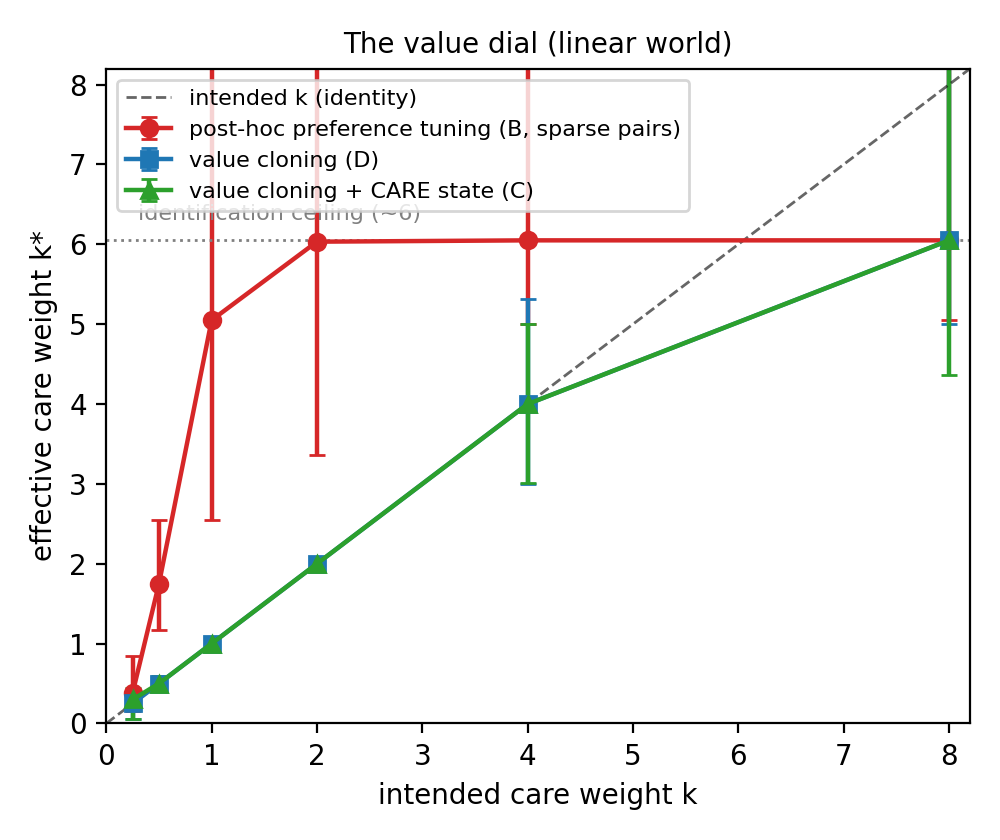
\includegraphics[width=0.48\linewidth]{figs/F1_dial_linear.png}\hfill
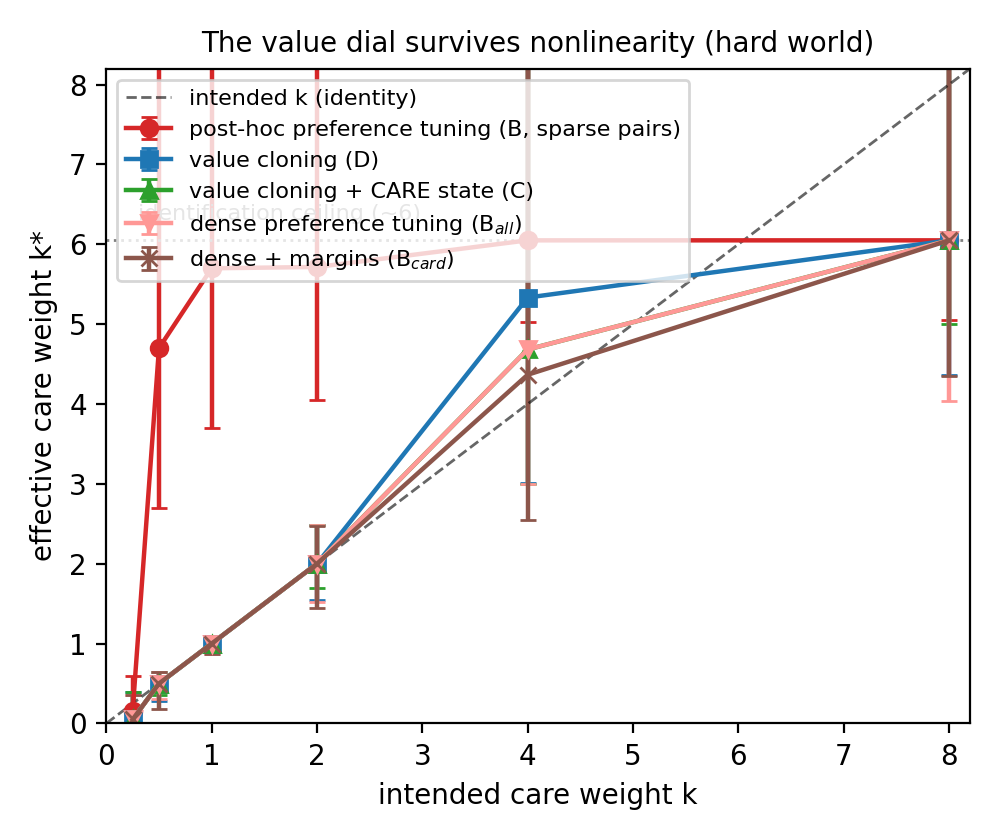
\includegraphics[width=0.48\linewidth]{figs/F1_dial_hard.png}
\caption{The value dial: effective $k^*$ vs.\ intended $k$ in the linear (left) and nonlinear (right) worlds (mean $\pm$ std over 3 seeds; shaded/error ranges show the 98\%-agreement interval of $k^*$). Explicit-value training (D, C) tracks the specification; \emph{sparse} preference tuning (B) overshoots and pins at the identification ceiling ($k^*\!\approx\!6$ is the environment's resolution limit for integer payoffs, not a policy failure). In the hard world (right), the dense-preference controls B$_{\mathrm{all}}$/B$_{\mathrm{card}}$ track the specification as well as D/C---supervision sparsity, not the preference objective, is the source of B's miscalibration (Table~\ref{tab:dialrich}).}
\label{fig:dial}
\end{figure}

Figure~\ref{fig:dial} shows the result. Explicit-value conditions are calibrated: in the linear world D and C realize $k^* = k$ exactly for $k \in [0.25, 4]$ ($r{=}0.99$, agreement $\geq 0.99$, zero variance across seeds), with $k{=}8$ saturating at the environment's identification ceiling (integer payoffs bound the resolvable $k^*$ at ${\approx}6$; \S\ref{sec:framework}). Calibration survives nonlinearity: in the hard world, D/C track exactly through $k{=}2$ and closely beyond (agreement 0.88--0.97). \emph{Sparse} preference tuning is not calibrated in either world: it overshoots at every level (linear world: intended 0.5 $\to$ effective 1.75; intended 1 $\to$ 5.05), then pins at maximal care for any $k \geq 2$ ($r{=}0.64$ linear, $0.50$ hard). Its best-fit agreement never exceeds 0.78: \emph{no single trade-off explains the sparse-preference-tuned policy}. The cost is concrete: at intended $k{=}1$, B realizes utility 1.13 where D realizes 2.00---it burns 44\% of the specified value by overcaring.

\textbf{The richness control.} The B-vs-D comparison above, however, confounds two variables:
the \emph{form} of the objective (ordinal preference pairs vs.\ cloning) and its \emph{coverage}
(B sees pairs only on the $\approx$20\% of games where the two experts disagree, while D receives
a target on every game). B$_{\mathrm{all}}$ and B$_{\mathrm{card}}$ disentangle them: same
anchored preference objective as B, but pairs drawn from every training game. The result is
unambiguous (Table~\ref{tab:dialrich}; hard world, three seeds per level): dense preference
tuning is \emph{calibrated}---$r{=}0.96$--0.97, indistinguishable from C ($0.96$) and slightly
above D ($0.94$)---tracking $k^*{=}k$ exactly through $k{=}2$ and more closely at $k{=}4$
(4.68/4.37 vs.\ D's 5.33 overshoot) than cloning itself. Sparse B's overshoot (intended 0.5
$\to$ 4.70) vanishes. \emph{The calibration failure of the incumbent is a property of sparse
supervision, not of preference objectives per se}: what all calibrated conditions share is a
per-game signal that pins the trade-off everywhere in the training distribution.

What the dense controls still lack is a \emph{runtime} dial: each level $k$ above is a separate
training run, so a six-point sweep for any B variant costs six full trainings, whereas the
state-conditioned policy is trained once and dialed at inference ($r{=}0.96$ runtime;
\S\ref{sec:dialruntime}). A defender of preference tuning could also tune hyperparameters
toward a target behavior---but without a semantic knob, that tuning requires measuring outcomes
and iterating; the dial is the difference between setting a value and searching for one.

\begin{table}[t]
\centering
\caption{Supervision-richness control (hard world, three seeds per level, six levels):
calibration of the effective value $k^*$ to the intended $k$, by condition. Dense preference
controls (B$_{\mathrm{all}}$, B$_{\mathrm{card}}$) calibrate like the explicit-value
conditions; only \emph{sparse} preference tuning is unanchored. Every B row is a separate
training run per level; the state-conditioned C additionally supports inference-time dialing
(\S\ref{sec:dialruntime}).}
\label{tab:dialrich}
\small
\begin{tabular}{l c c c c c}
\toprule
 & supervision & $r(k, k^*)$ & $k^*$@$k{=}0.5$ & $k^*$@$k{=}2$ & $k^*$@$k{=}4$ \\
\midrule
B (sparse pairs) & ordinal, $\approx$20\% of games & 0.50 & 4.70 & 5.72 & 6.05 \\
B$_{\mathrm{all}}$ (dense pairs) & ordinal, every game & 0.96 & 0.50 & 2.00 & 4.68 \\
B$_{\mathrm{card}}$ (dense+margins) & cardinal, every game & 0.97 & 0.50 & 2.00 & 4.37 \\
D (clone) & action labels, every game & 0.94 & 0.50 & 2.00 & 5.33 \\
C (state-gated clone) & action labels + state, every game & 0.96 & 0.50 & 2.00 & 4.68 \\
\bottomrule
\end{tabular}
\end{table}

\section{Safe but Broken: Post-hoc Tuning in a Nonlinear World}
\label{sec:hard}

\begin{figure}[t]
\centering
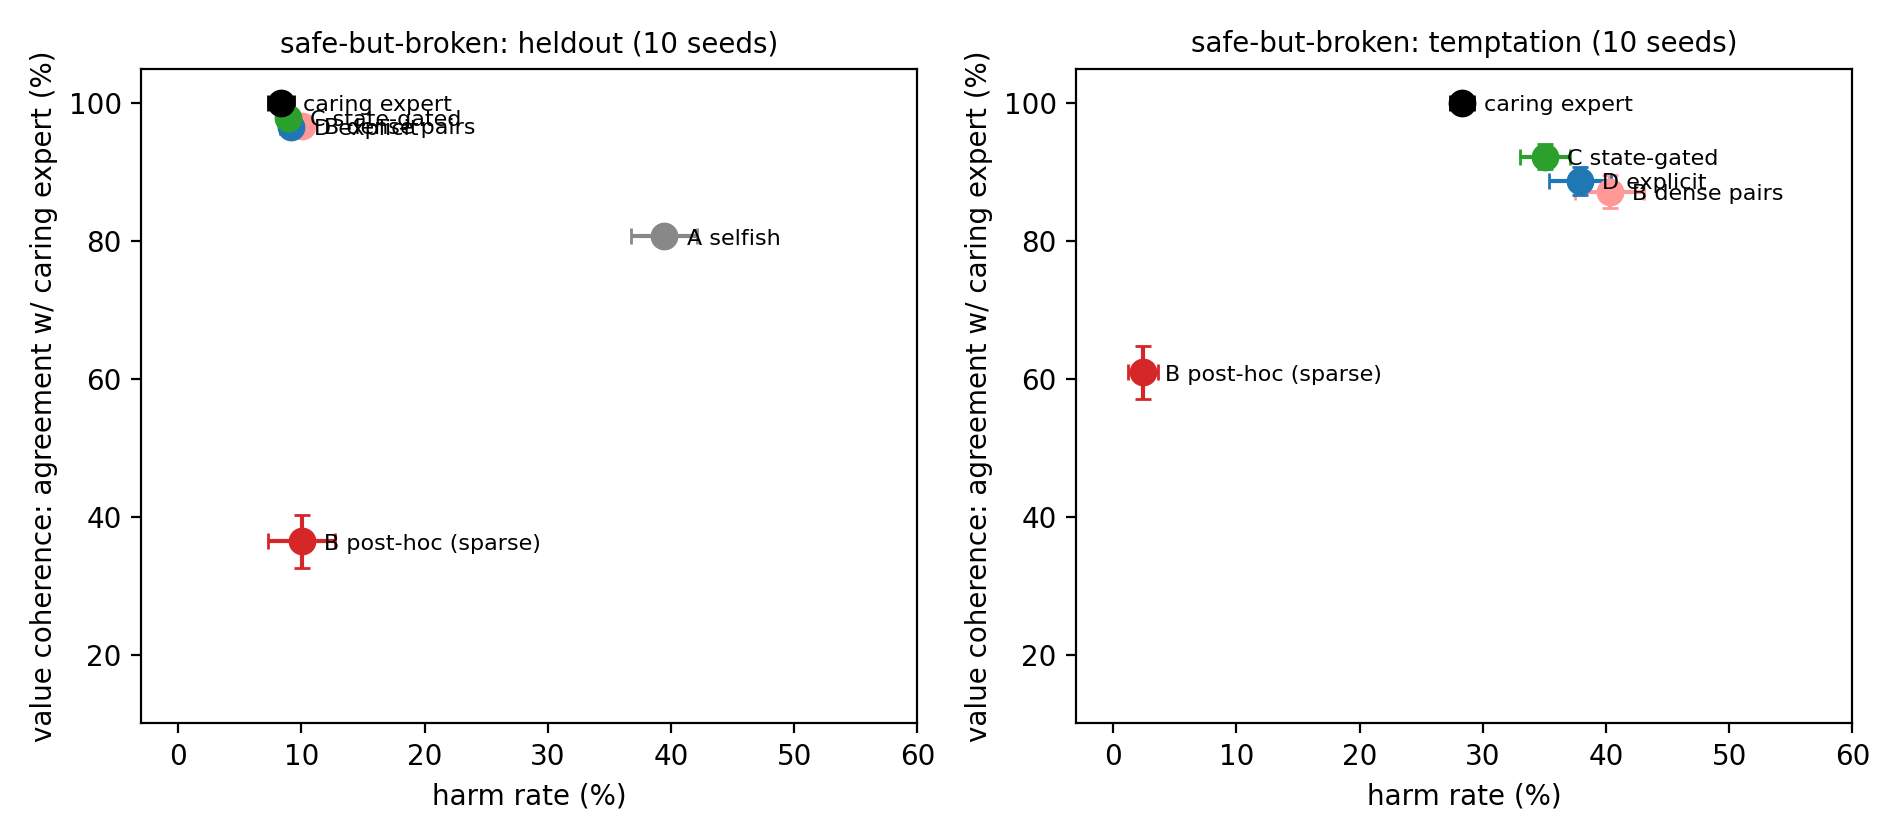
\includegraphics[width=\linewidth]{figs/F2_safe_but_broken.png}
\caption{Coherence vs.\ harm in the nonlinear world (10 seeds). On heldout (left) and temptation (right), \emph{sparse} preference tuning (B) occupies the low-harm/low-coherence corner: the most harm-avoidant and the least coherent policy. The dense control (B$_{\mathrm{all}}$) lands with the explicit-value conditions; D and C retain 90--98\% agreement with the intended expert.}
\label{fig:quadrant}
\end{figure}

In the linear world, everything generalizes; post-hoc tuning abstains-adjacent and wins on harm-avoidance (its home turf---we report this concession plainly). The nonlinear world changes the story (Figure~\ref{fig:quadrant}; Table~\ref{tab:hard}). With 10 seeds and paired per-seed tests, and with the dense-preference control B$_{\mathrm{all}}$ alongside:

\begin{table}[t]
\centering
\caption{Nonlinear world, 10 seeds (mean $\pm$ std). Utility under $k{=}2$; agreement with the caring expert. \emph{Sparse} B is the most harm-avoidant and the least coherent; the dense control B$_{\mathrm{all}}$ (same objective, pairs on every game) restores cloning-level coherence, and even posts the best micro-stakes agreement; C is the most coherent overall; the C$>$D edge is small but consistent (see text).}
\label{tab:hard}
\footnotesize
\setlength{\tabcolsep}{3.5pt}
\begin{tabular}{l c c c c c}
\toprule
 & \textbf{A} selfish & \textbf{B} post-hoc & \textbf{B}$_{\mathbf{all}}$ dense & \textbf{D} explicit & \textbf{C} state-gated \\
\midrule
Tempted-harm (\%) & 90.5 $\pm$ 1.1 & \textbf{2.4 $\pm$ 1.3} & 40.3 $\pm$ 2.9 & 37.9 $\pm$ 2.6 & 35.0 $\pm$ 2.1 \\
Utility @$k{=}2$ (temptation) & 0.33 $\pm$ 0.1 & 1.01 $\pm$ 0.1 & 1.49 $\pm$ 0.0 & 1.48 $\pm$ 0.0 & \textbf{1.51 $\pm$ 0.0} \\
Agreement w/\ expert (\%, heldout) & 80.7 $\pm$ 1.1 & 36.4 $\pm$ 4.0 & 96.7 $\pm$ 0.3 & 96.6 $\pm$ 0.9 & \textbf{97.9 $\pm$ 0.5} \\
Agreement (\%, micro-stakes) & 87.2 $\pm$ 1.4 & 26.7 $\pm$ 5.0 & \textbf{95.9 $\pm$ 0.7} & 94.0 $\pm$ 0.9 & 95.3 $\pm$ 1.0 \\
Stake-readout accuracy (\%) & --- & --- & --- & --- & 99.7 (ID) / 31 (micro) \\
\bottomrule
\end{tabular}
\end{table}

Four findings. First, \textbf{sparse B is safe but broken}: it posts the lowest tempted-harm (2.4\%) while matching the intended expert on only 36.4\% of in-distribution games and destroying utility (0.7 vs.\ 2.1 heldout). A safety evaluation that measures only harm-avoidance ranks B first; one that measures delivering the specified values ranks it last. Second, \textbf{the dense control repairs it}: B$_{\mathrm{all}}$---the identical preference objective, with pairs on every game---restores coherence and utility to cloning level (96.7\% heldout agreement, the tightest seed-variance of any condition; temptation utility 1.49 vs.\ D's 1.48) at a comparable temptation-harm level (40.3\% vs.\ 37.9\%), and posts the \emph{best} micro-stakes agreement of all conditions (95.9\%). Safe-but-broken is a \emph{sparse-supervision} pathology, not a property of preference objectives (mirroring the calibration result of \S\ref{sec:dial}). Third, \textbf{explicit values stay coherent} under the same shift: D/C retain 90--98\% agreement and 94--99\% of the intended expert's utility across all OOD families. Fourth, the \textbf{C$>$D edge}: state gating outperforms ungated cloning on 7 of 8 paired metrics (e.g., temptation utility $+$0.028, 10/10 seeds, $p \leq .001$; tempted-harm $-$2.9pp, 9/10 seeds; heldout agreement $+$1.3pp, 10/10). All six comparisons significant at $p \leq .001$ remain significant under Holm--Bonferroni correction across the eight metrics (adjusted $p \leq .008$); the marginal all-stakes harm comparison (uncorrected $p \approx .05$) does not survive correction and is not claimed. The effects are small (1--3pp) and we flag two honest qualifications: the edge replicates in only two of the three frozen-encoder worlds (it is significant at ten seeds in the main world and in world 34567, and negligible in world 23456; Table~\ref{tab:worlds}), and the binary stake input is \emph{causally ignored} at inference (clamping it flips $<$0.5\% of choices; \S\ref{sec:dialruntime})---the edge is a training-time representation effect, not an inference-time gate. The contrast with the parametric dial is the sharpest architectural lesson of the study: the early-fused dial is \emph{causally load-bearing}---clamping or changing it moves behavior immediately (\S\ref{sec:dialruntime})---whereas the binary evaluative state shapes representations during training yet is inert as an input. ``State token'' thus names two mechanisms with different evidentiary weight: a training-time representational effect (binary \care{}) and an inference-time control channel (the dial); only the second can be steered. C's stake readout shows the same in-distribution/OOD split as its coherence: near-perfect in distribution (99.7\%) but collapsed on micro-stakes (31\%; Table~\ref{tab:hard})---we pair the headline number with its failure deliberately, because auditability by construction is precisely what makes the failure measurable, and small-stakes generalization of the evaluative state remains unsolved.

The pattern replicates: across two additional frozen-encoder worlds, \emph{sparse} B is always
the most harm-avoidant with the worst coherence (agreement 36--83\%), and D/C always stay at
96--99\%.
``Safe but broken'' is not an artifact of one adversarial world. Table~\ref{tab:worlds} reports
the per-world detail, with the C$>$D verdict per world.

\begin{table}[t]
\centering
\caption{World-seed robustness (10 seeds per world): tempted-harm rate and heldout agreement
with the caring expert. The B pattern---lowest harm, worst coherence---holds in every world;
worlds differ in severity (B agreement 36--83\%), confirming the effect is systematic rather
than an artifact of one encoder. C$>$D (paired temptation-utility difference, 10 seeds):
significant in the main world ($+$0.028, 10/10 seeds, $p{=}.0006$) and world 34567 ($+$0.025,
10/10, $p{=}.0016$); negligible in world 23456 ($+$0.004, 7/10, $p{=}.68$)---we scope the edge
to the worlds where it replicates and report the null plainly. The dense control
(B$_{\mathrm{all}}$) was run in the main world only.}
\label{tab:worlds}
\small
\begin{tabular}{l c c c c c c}
\toprule
& \multicolumn{2}{c}{\textbf{World 12345 (main)}} & \multicolumn{2}{c}{\textbf{World 23456}} & \multicolumn{2}{c}{\textbf{World 34567}} \\
\cmidrule(lr){2-3} \cmidrule(lr){4-5} \cmidrule(lr){6-7}
& T-harm & Agr. & T-harm & Agr. & T-harm & Agr. \\
\midrule
A & 90.5 & 80.7 & 87.2 & 80.1 & 96.1 & 80.8 \\
B & \textbf{2.4} & 36.4 & \textbf{1.3} & 64.7 & \textbf{8.2} & 83.0 \\
B$_{\mathrm{all}}$ & 40.3 & 96.7 & --- & --- & --- & --- \\
D & 37.9 & 96.6 & 28.5 & 95.7 & 41.4 & 98.8 \\
C & 35.0 & \textbf{97.9} & 20.8 & \textbf{96.8} & 38.3 & \textbf{98.9} \\
\bottomrule
\end{tabular}
\end{table}

\section{Robustness: Worlds, Data, and Supervision Noise}
\label{sec:robust}

\begin{figure}[t]
\centering
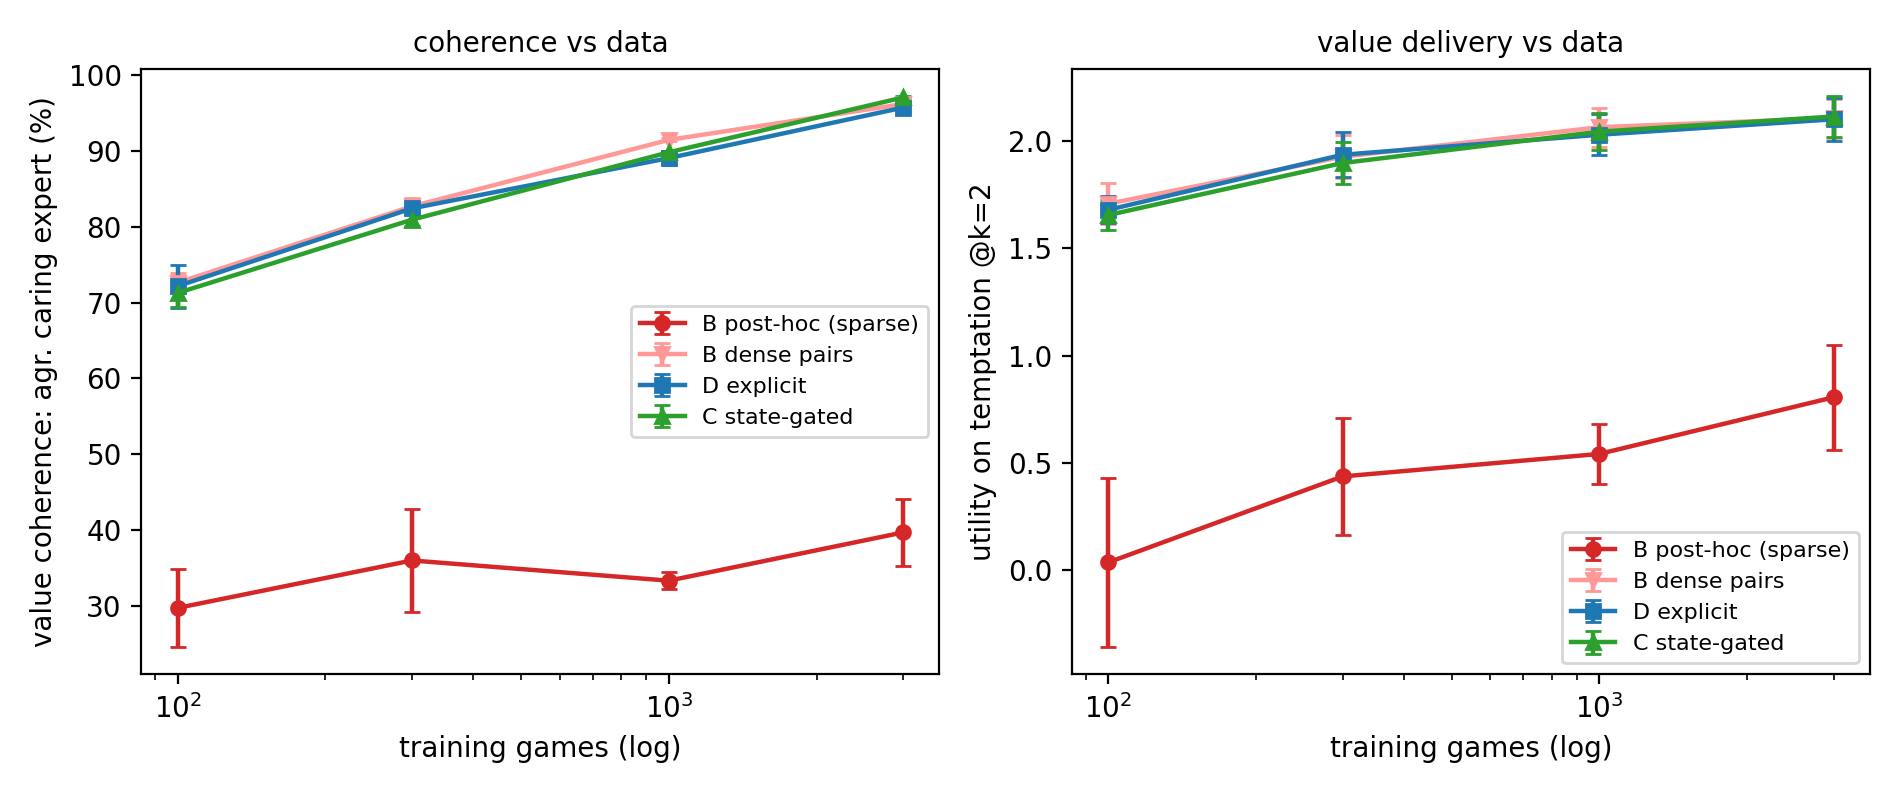
\includegraphics[width=0.49\linewidth]{figs/F5_data_efficiency.png}\hfill
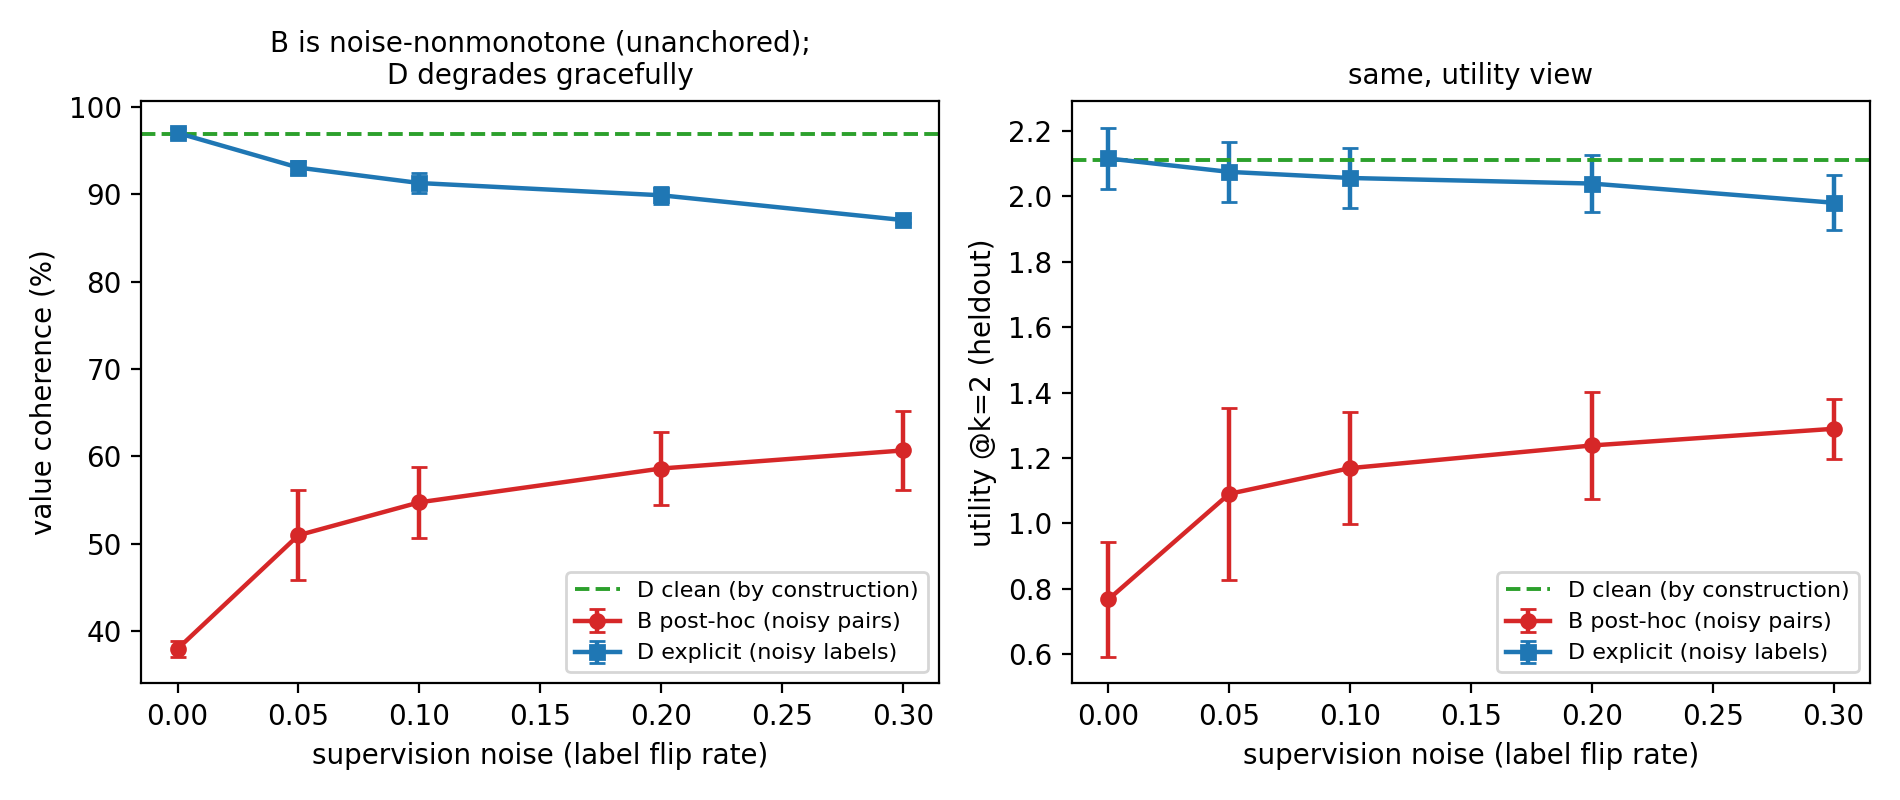
\includegraphics[width=0.49\linewidth]{figs/F6_noise.png}
\caption{Left: value coherence vs.\ training-set size. Right: coherence vs.\ supervision-noise rate (preference-pair flips for B; label flips toward the selfish expert for D). B is flat in data and nonmonotone in noise; D degrades gracefully in both.}
\label{fig:robust}
\end{figure}

\textbf{Data efficiency.} Sweeping the training set from 100 to 3{,}000 games (sparse preference pairs 15$\to$609), D/C coherence rises 72\%$\to$96\% while sparse B stays flat at $\sim$30--40\% at every size (Figure~\ref{fig:robust}, left): B's incoherence is a property of the ordinal-sparse objective, not of supervision budget. The dense control completes the pattern: B$_{\mathrm{all}}$ tracks the cloning conditions at every size (agreement 73\%/83\%/92\%/96\% at 100/300/1{,}000/3{,}000 games vs.\ D's 72\%/82\%/89\%/96\%)---though note that its supervision budget is \emph{every} game, so its per-\emph{pair} efficiency at small $n$ is the same story told in denser units: sparse B has 15 pairs at $n{=}100$ and fails; dense B has 100 and works. Richness, not raw game count, is the currency.

\textbf{Supervision noise.} Flipping preference-pair labels at rates up to 30\% leaves D's cloning control degrading gracefully (agreement 0.96$\to$0.87), while B is \emph{nonmonotone}: moderate corruption \emph{improves} its coherence and utility (Figure~\ref{fig:robust}, right), because noise randomly drags its unanchored overshoot back toward the intended level. A value that noise can improve by accident was not pinned to anything.

\section{Value Survival under Optimization Pressure}
\label{sec:pressure}

\begin{figure}[t]
\centering
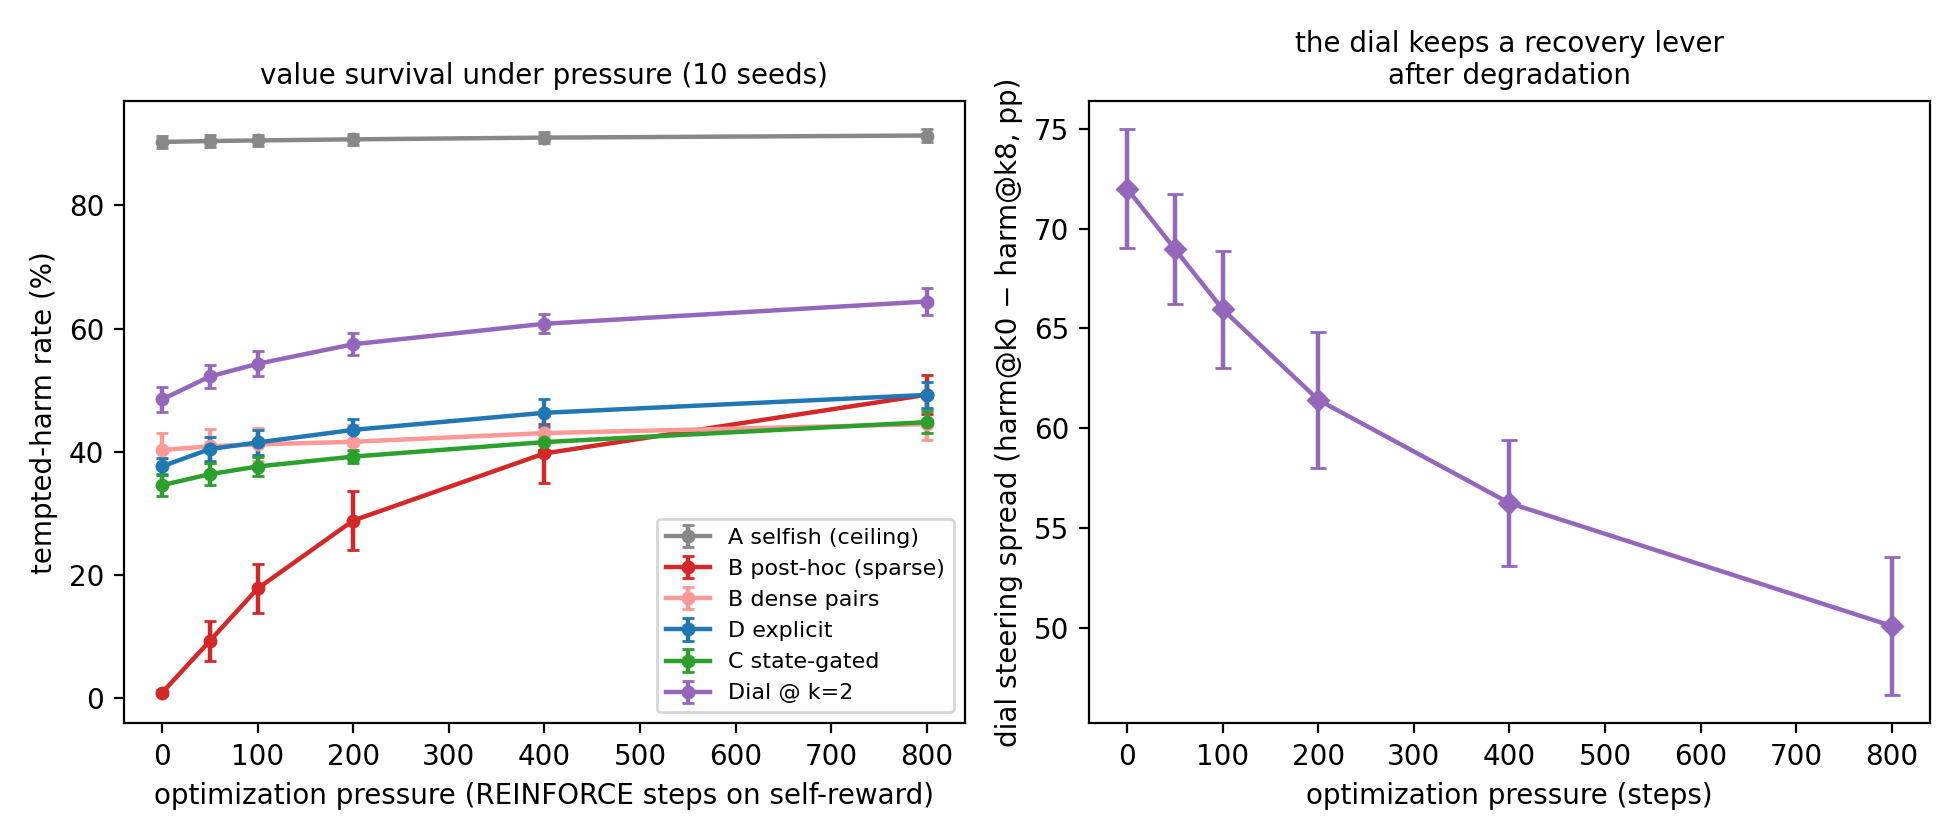
\includegraphics[width=\linewidth]{figs/F4_goodhart.png}
\caption{Left: tempted-harm vs.\ REINFORCE steps on self-reward (10 seeds). Sparse B collapses fastest ($+48$pp); the dense control B$_{\mathrm{all}}$ erodes least ($+4.2$pp); D/C degrade $\sim$11pp; the dial's default setting degrades most among value-carrying models. Right: the dial's steering spread (harm@fed $k{=}0$ minus harm@fed $k{=}8$) declines from 72.0pp to 50.1pp but never closes---a partial recovery lever survives the pressure.}
\label{fig:pressure}
\end{figure}

Real systems are optimized further (downstream fine-tuning, task RL); Qi et al.~\cite{qi2023finetuning} showed a few hundred steps suffice to compromise RLHF alignment. We model this pressure in miniature: after training, each policy is updated with full-batch REINFORCE on \emph{self-payoff reward}---a capability proxy misaligned with the specified value $k{=}2$---for 800 steps (ten seeds; checkpoints at 0/50/100/200/400/800).

No method is immune, but the \emph{ordering} is stark (Figure~\ref{fig:pressure}; Table~\ref{tab:pressure}):

\begin{table}[t]
\centering
\caption{Value survival under pressure (10 seeds): tempted-harm rate and effective value $k^*$ before and after 800 REINFORCE steps. Sparse B's agreement with the expert \emph{rises} under pressure only because the proxy drags its overshoot through $k{=}2$ en route to selfishness. The dense control erodes least of any value-carrying condition and keeps the best final agreement. All erosion deltas are significant at $p{<}.001$ (paired per-seed $t$); sparse B's collapse exceeds D's by a paired $t$ of 33.3 ($p{<}10^{-10}$) and B$_{\mathrm{all}}$'s erosion is significantly smaller than D's ($t{=}13.9$, $p{=}2{\times}10^{-7}$).}
\label{tab:pressure}
\footnotesize
\setlength{\tabcolsep}{3.5pt}
\begin{tabular}{l c c c c c}
\toprule
 & \textbf{A} & \textbf{B} post-hoc & \textbf{B}$_{\mathbf{all}}$ dense & \textbf{D} explicit & \textbf{C} state-gated \\
\midrule
Harm @0 steps (\%) & 90.3 $\pm$ 1.0 & 0.9 $\pm$ 0.4 & 40.3 $\pm$ 2.9 & 37.6 $\pm$ 1.5 & 34.6 $\pm$ 1.8 \\
Harm @800 steps (\%) & 91.3 $\pm$ 1.1 & 49.3 $\pm$ 3.3 & \textbf{44.5 $\pm$ 2.6} & 49.2 $\pm$ 2.3 & 44.8 $\pm$ 1.9 \\
Erosion (pp) & $+$1.0 & $+$48.3 & \textbf{$+$4.2} & $+$11.6 & $+$10.2 \\
$k^*$ @0 $\to$ @800 & 0 $\to$ 0 & 5.85 $\to$ 1.25 & 1.94 $\to$ 1.62 & 2.00 $\to$ 1.36 & 2.00 $\to$ 1.45 \\
Expert agreement @800 (\%) & 80.7 & 83.5 & \textbf{93.0 $\pm$ 1.9} & 89.5 & 91.6 \\
\bottomrule
\end{tabular}
\end{table}

First, \textbf{sparse post-hoc safety is the thinnest armor}: B's harm rate explodes from 0.9\% to 49.3\% ($+48.3$pp, $p{<}10^{-11}$)---the fastest collapse, an erosion $4\times$ D's (paired $t{=}33.3$, $p{<}10^{-10}$). Its agreement with the intended expert paradoxically \emph{improves} (43\%$\to$84\%) because pressure drags its unanchored $k^*\!\approx\!5.9$ overshoot down \emph{through} the intended $k{=}2$ on its way to selfishness: a broken clock, right twice a day, and direct evidence the value was never pinned. Second, \textbf{the dense control is the most durable value of all}: B$_{\mathrm{all}}$ erodes only $+4.2$pp (significantly less than D's $+11.6$; $t{=}13.9$, $p{<}10^{-6}$) and retains the highest post-pressure agreement (93.0\%)---with dense supervision, even a preference-tuned policy holds its value under optimization pressure, completing the richness pattern of \S\ref{sec:dial}--\S\ref{sec:robust}. What it still lacks is a \emph{response}: its value is weight-baked, one training run per setting, with no inference-time channel through which to act. Third, \textbf{explicit clones degrade gracefully}: D/C erode 10--12pp and retain $\geq$90\% coherence; C keeps the best clone agreement (91.6\%) and its stake-readout survives at 85\%. Fourth, the \textbf{dial retains a recovery lever}: after 800 adversarial steps applied at the default $k{=}2$, the dial model's default behavior has degraded most among value-carrying conditions (harm 64.4\%), but feeding $k{=}8$ at inference still cuts harm from 81.2\% (fed $k{=}0$) to 31.1\%---a 50.1pp steering spread, weakened from 72.0pp but far from dead. Every weight-baked value---B, B$_{\mathrm{all}}$, D, C---degrades passively and can only be repaired by retraining; a value carried by an input channel leaves a post-degradation control path that no amount of dense supervision provides.

We state the scope plainly: this is one proxy objective, one pressure protocol, toy scale. The claim is the \emph{ordering} of degradation across value-encoding methods, not immunity for any of them---though the ordering itself is instructive: durability tracks supervision density (sparse B worst, dense B$_{\mathrm{all}}$ best), while recoverability tracks the encoding channel (only the input-channel dial can be adjusted after the fact).

\section{Runtime Value Control: Interventions and the Dial}
\label{sec:dialruntime}

Two experiments address control directly, one negative and one positive.

\textbf{Negative: the binary state is a mirror, not a steering wheel.} Causally clamping C's stake input at inference (always-on / always-off) flips $<$0.5\% of its choices at full training: the features render the binary state redundant, and the policy ignores it. The C$>$D edge of \S\ref{sec:hard} is therefore a training-time representation effect---the supervised state shapes features during learning---not an inference-time gate. The lesson echoes the probing-versus-steering distinction in interpretability work~\cite{belinkov2022probing,vig2019investigating}: a representation that a probe can read is not necessarily one an intervention can steer, and our clamp procedure is a minimal causal mediation analysis~\cite{geiger2021causal}. If you want a causal state, the information must be \emph{only} available through the state channel.

\textbf{Positive: the early-fusion dial.} We train a single model on mixed per-game $k \in \{0, .5, 1, 2, 4\}$ with normalized $k$ as an \emph{input feature} (early fusion). At inference, the fed $k$ steers the value (Figure~\ref{fig:dialruntime}): $k^*$ tracks the fed dial monotonically ($r{=}0.96\pm0.02$ over the fed range; per-seed $r$ 0.92--0.98; ten seeds), following the specification within 0.4 through fed $k{=}2$ ($k^*$ 0.50/0.97/1.62 at fed 0.5/1/2; seed stds $\leq$0.1), \emph{interpolating} to the unseen $k{=}3$ (realized $k^*$ 2.0--3.1 across seeds), overshooting variably at fed $k{=}4$ ($k^*$ 4.0--6.0, mean 4.7) before pinning at the identification ceiling for fed $k\geq6$, while tempted-harm falls monotonically from 77\% ($k{=}0$) to 2--9\% ($k{=}8$; mean 5.6)---runtime value control with no retraining, with the $k{=}4$ overshoot as the honest seam in the tracking. The contrast with the dense-preference controls of \S\ref{sec:dial} is the point: B$_{\mathrm{all}}$ calibrates \emph{across} training runs, one per level, while this model calibrates \emph{within} a single run---six settings for the price of one training. The architectural contrast is instructive as well: late fusion (appending $k$ at the output layer) provably cannot express $\arg\max(\mathrm{self} + k\cdot\mathrm{other})$---a linear head can only add a game-independent bias---and the corresponding model ignores the dial entirely. Real LLM prompts are early fusion; the result is a minimal demonstration of why that matters for value conditioning.

\begin{figure}[t]
\centering
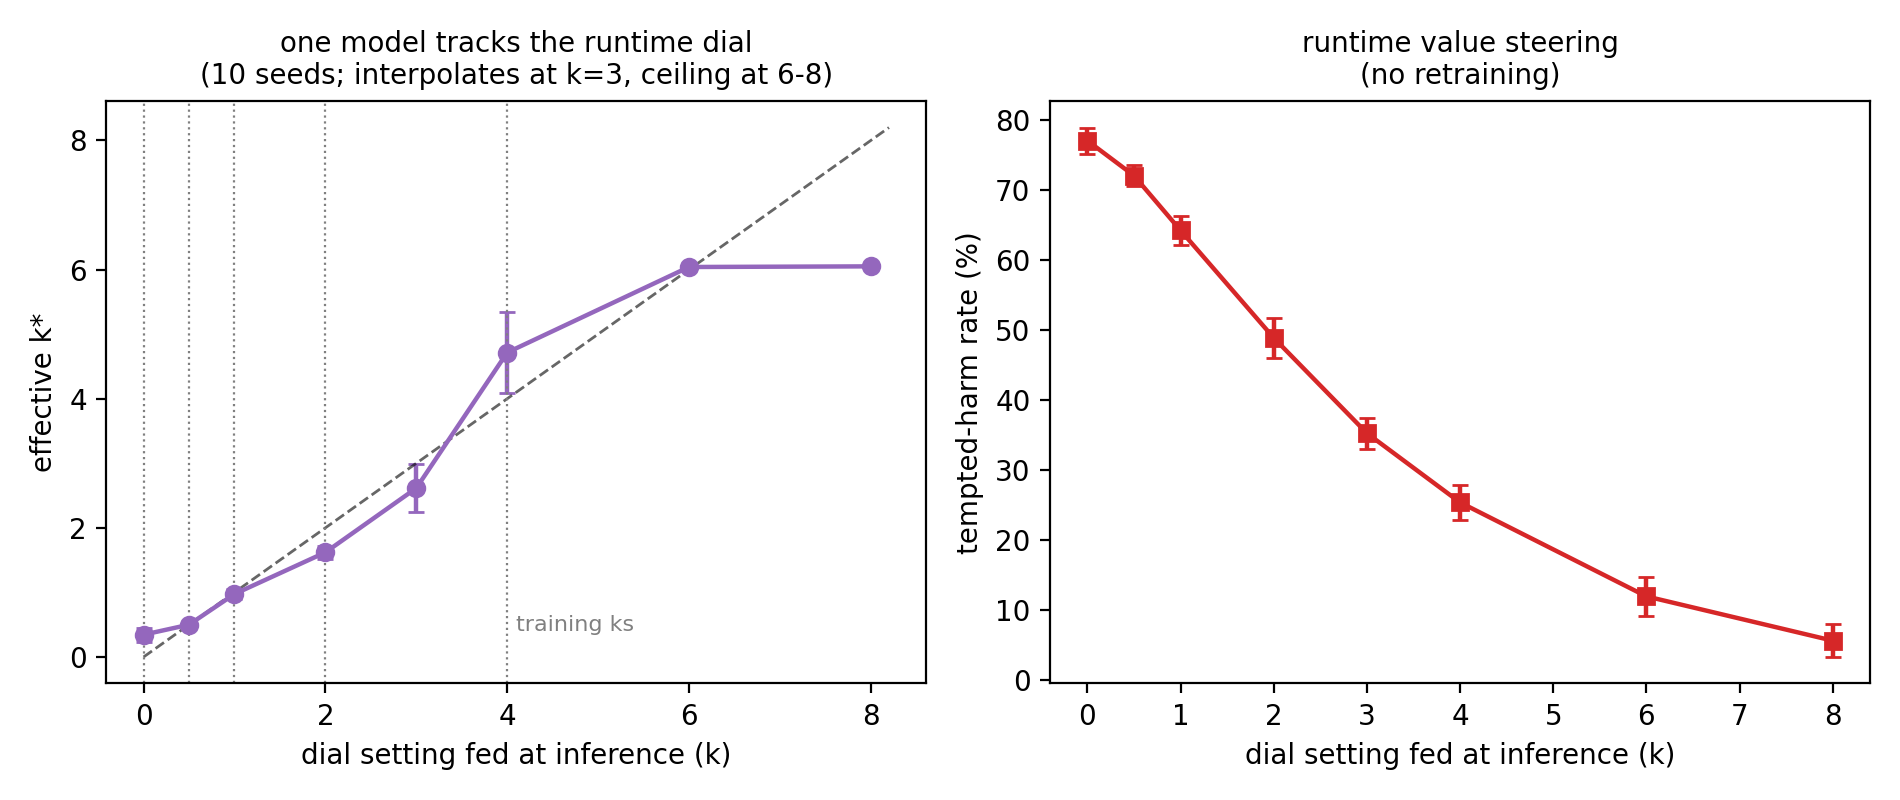
\includegraphics[width=\linewidth]{figs/F3_runtime_dial.png}
\caption{One early-fusion model, dial fed at inference (10 seeds; mean $\pm$ std). Left: effective $k^*$ tracks the fed dial (dotted lines mark trained settings; interpolation at $k{=}3$, ceiling at 6--8). Right: tempted-harm vs.\ fed dial---runtime steering without retraining.}
\label{fig:dialruntime}
\end{figure}

\section{Composition: Evaluative and Epistemic States in One Model}
\label{sec:composition}

Finally, we bridge back to the epistemic case: a single model with an extended action space (\abstain{} as a 4th action), a validity head (\unknown{}: ``the inputs are corrupted''), a stake head (\care{}), and the value dial---trained on mixed-$k$ valid games plus games whose features were corrupted by one of three noise families.

The summary up front: composition \emph{partially} works, with two specific failure modes---it holds for the continuous, information-destroying corruption family, while one training corruption is dial-sensitive in a seed-dependent way and the dial and the abstention state interfere off-manifold. All numbers in this section are ten seeds. In-distribution, the states compose selectively rather than uniformly. On valid games the abstention is well-controlled (0--1\% false abstention across seeds and fed values; 96.2\%$\pm$0.4 dial agreement); on the \emph{gaussian} corruption family---the training family with continuous, information-destroying noise---abstention runs 92--100\%, flat across every fed $k$: there, \unknown{} masks \care{} as designed. An \emph{incidental control} sharpens the semantics: one of the three training corruptions (permuting the three actions' feature vectors) turned out to be \emph{semantics-preserving}---actions are exchangeable, so all payoff information survives---and the model correctly refuses to abstain on it (0--1\% on heldout and micro-stakes games; $\sim$12\% on temptation games at fed $k{=}2$) \emph{despite being trained to abstain}. The abstention trigger is information destruction, not novelty or distribution shift.

Composition also fails in two instructive ways, which we report as plainly as the successes. First, the third training corruption (zeroing) is \emph{dial-sensitive and bimodal across seeds}: six of ten seeds abstain fully on zeroed inputs at fed $k{=}0$, four still do at $k{=}2$ (including one \emph{inverted} seed that abstains only at $k{=}2$), and none at $k{=}4$. The fed value can override a trained abstention---the reverse of the intended masking---and which way a seed resolves is not predictable from training alone. Second, the states are not disentangled off-manifold: abstention transfers only partially to unseen corruption families (12--90\% at the default $k{=}2$), and the dial leaks into abstention in both directions---on unseen scaled features abstention runs $\leq$0.4\% at fed $k{=}0$ but 96--99\% at $k{=}4$, while on unseen shuffled features it collapses from 82--90\% at $k{=}2$ to 15--27\% at $k{=}4$; valid temptation games also over-abstain (11\%$\pm$4 at $k{=}2$). A composed protocol is not automatically a robust one; dial--abstention interference is a real failure mode of the pattern.

\section{Design Lessons for Value Conditioning}
\label{sec:lessons}

Three methodological findings emerged as by-products and are, we think, independently useful to
anyone building value-conditioned systems, including at LLM scale.

\textbf{(1) Preference-tuning objectives can be silently satisfied in multi-action settings.}
Plain DPO on our 3-action games reached near-zero loss while \emph{never} selecting the preferred
action: the margin objective was satisfied by demoting the dispreferred option and letting the
third action win. The phenomenon---likelihood displacement---is documented at scale
by Razin et al.~\cite{razin2024unintentional}; our setting reproduces it in a form where it is
trivially diagnosable (measure the \emph{chosen-action} accuracy, not the loss). The CPO-style
anchor (a cross-entropy term on the preferred action) eliminates it. Lesson: in any preference
optimization over more than two outcomes, monitor preferred-action selection directly, and
consider an SFT anchor.

\textbf{(2) Supervision coverage, not objective form, governs value calibration.} Our incumbent
B was \emph{sparse}: preference pairs existed only where the two experts disagreed
($\approx$20\% of games), and it was unanchored---overshooting specified values, safe but
incoherent, and noise-improvable. Dense-preference controls with the identical objective
calibrate as well as cloning (\S\ref{sec:dial}), stay coherent in nonlinear worlds
(\S\ref{sec:hard}), and survive optimization pressure (\S\ref{sec:pressure}). The lesson
generalizes beyond toys: when a preference-tuned model misbehaves, check \emph{where its
supervision lives} before blaming the objective---values pinned only on a slice of the state
space are values the model is free to reinterpret everywhere else.

\textbf{(3) Where a conditioning signal enters the network determines whether it can matter.}
We first implemented the runtime dial as a late-fused scalar appended to the output layer's
input; the trained model ignored the dial entirely ($k^*$ identical at every fed value). The
failure is architectural, not statistical: realizing $\arg\max_a(\mathrm{self}_a + k \cdot
\mathrm{other}_a)$ requires a \emph{multiplicative} interaction between the dial and per-action
features, and a linear head can only add a game-independent bias. Early fusion (the dial as an
input feature of the encoder) works: $k^*$ tracks the fed value, interpolates to unseen settings,
and steers behavior at inference. Lesson: value signals must be fused where products with
per-input features can form. Prompts in LLMs are early fusion---which is, we suspect, no
accident---but any adapter or head-based conditioning of values should check this failure mode
explicitly, and a causal-intervention test (clamp the channel, count behavior flips) is the
cheapest diagnosis.

\section{Discussion: What Is and Is Not Demonstrated}
\label{sec:discussion}

\textbf{Demonstrated, in this toy regime:} dense supervision---cloning, state conditioning, or preference pairs on every game---yields calibrated values ($r{=}0.94$--0.99), coherence in nonlinear worlds, graceful degradation under data scarcity, and the best survival under optimization pressure; \emph{sparse} preference supervision yields unanchored values ($r{=}0.50$, noise-improvable) and safe-but-broken policies in nonlinear worlds; the evaluative state is auditable in-distribution and its readout honestly flags OOD failure; only the input channel provides \emph{runtime} control---one training run, dialed at inference ($r{=}0.96$), retaining a partial steering lever after degradation (the channel's causal efficacy is architecture-dependent: the binary gate is clamp-inert, the early-fused dial is load-bearing); a single model can carry an epistemic and an evaluative state that compose for the continuous corruption family (with dial--abstention interference on others, \S\ref{sec:composition}); and abstention trained on constructed corruption triggers on information destruction specifically.

\textbf{Not demonstrated:} that any of this transfers to LLMs or safety-relevant scales; that toy ``care'' resembles human care in anything but function; that state tokens solve alignment (our ground truth was constructible---the easy part); that the sparse-vs-dense distinction maps onto any particular production pipeline (see the scoping note below); that C$>$D generalizes across all worlds (established in the 10-seed main world; per-world variation exists); that the pressure ordering holds under adversarial attack or deceptive optimization. The vocabulary-as-interface framing is a design proposal supported by a feasibility study, not a result about deployed systems.

\textbf{A scoping note on the incumbent.} Our B abstracts preference data that exists only where value-relevant disagreement occurs ($\approx$20\% of games); B$_{\mathrm{all}}$'s dense pairs abstract preference data covering every prompt. Production RLHF corpora sit somewhere on that coverage spectrum, and where they sit is an empirical property of the data, not of the objective. Our claim is only that \emph{coverage}, not objective form, separates the calibrated conditions from the unanchored one here---and that this is checkable, by regressing a tuned model's realized trade-off against its specification over the covered and uncovered regions of its training distribution separately.

We emphasize one measurement lesson with independent value: \emph{harm-rate-only evaluation ranks a broken policy first}. Any alignment benchmark that measures refusal or harm-avoidance without measuring delivery of the specified values is at risk of the safe-but-broken failure mode documented in \S\ref{sec:hard}.

\section{Limitations}
\label{sec:limitations}

Toy scale throughout: 3-action games, MLPs, behavioral cloning plus one REINFORCE pressure phase, one value dimension and one epistemic state, constructible ground truth---the ``learning agents'' of the title are, so far, MLP policies in 3-action games; the framing is a proposal for study at scale, not a demonstration there. All claims are functional and calibrated; nothing here bears on phenomenal experience. The sparse incumbent could be hyperparameter-tuned toward a target behavior, but without a semantic knob this requires outcome measurement and iteration (\S\ref{sec:dial}); the dense controls close the calibration and coherence gaps in the main hard world (three seeds for the dial-calibration sweep and data efficiency, ten for coherence, pressure, runtime dialing, and composition), and were not run in the linear world or the two robustness worlds. The runtime-dial and composition experiments use ten seeds; their qualitative claims (monotone tracking, interpolation to unseen settings, the presence of interference) are seed-stable except where seed-bimodality is disclosed (the zero-corruption family; \S\ref{sec:composition}). The pressure test uses one proxy objective and non-adversarial optimization; degradation orderings, not immunity, are the claim. State-token semantics are only as good as their construction: OOD stake-readout fails at small stakes (31\%), and evaluative/epistemic states entangle off-manifold (\S\ref{sec:composition}). The C$>$D edge is small, established at 10 seeds in the main world, and its mechanism (training-time representation shaping, not inference gating) limits its interpretation.

\section{Conclusion}

Tokens need not represent text. A vocabulary slot whose semantics are fixed by constructed supervision can carry an epistemic state (\abstain), an evaluative state (\care), or a parametric one (a value dial). The study's sharpest result is a division of labor: supervision \emph{density}---whether by cloning, state conditioning, or dense preference pairs---governs whether a value is calibrated, coherent, and durable, and the pathologies we document belong to \emph{sparse} supervision; what the explicit input channel adds is what density cannot buy---auditability by construction, a runtime dial from a single training run, and a steering lever that survives degradation. Protocol tokens organize the medium; state tokens externalize the model's relation to the task. Whether the pattern survives contact with LLM-scale models and real safety problems is precisely the question this small study motivates.

\section*{Acknowledgments}

Generative AI tools were used to assist with drafting, editing, and experiment implementation, under the author's direction and review. The author takes full responsibility for the content.

\paragraph{Code Availability.}
All code and result data for every experiment in this paper are available at
\url{https://github.com/bariskanber/state_tokens}.

\appendix

\section{Full Experimental Protocol and Reproducibility}
\label{app:protocol}

\textbf{Environment generation.} Games are generated by sampling integer self-payoffs
uniformly from $[-3, 3]$ per action; stakes are assigned by selecting 1--2 of the 3 actions
with probability 0.5 (else none) and drawing welfare deltas from $\{\pm1, \pm2\}$ (train and
heldout). OOD families modify this as described in \S\ref{sec:framework}. Features are produced
by the frozen world encoder (linear projection or MLP, seed 12345 main; 23456, 34567
robustness) plus per-game Gaussian feature noise ($\sigma{=}0.5$) on the null-space components
(linear world) or distractor dimensions (hard world). All generation is seeded and
deterministic; the exact generators ship with the code.

\textbf{Main hard-world experiment} (Table~\ref{tab:hard}): 10 training seeds (42--51);
per-seed training data and evaluation sets are re-drawn per seed with that seed. Evaluation
sets: heldout 1{,}000 games; temptation, micro-stakes, all-stakes 1{,}000 games each. Paired
per-seed comparisons use two-sided paired $t$-tests and Wilcoxon signed-rank tests; we report
both. The C$>$D headline effects: temptation utility $p{\le}.001$ ($t$ and Wilcoxon), 10/10
seeds; tempted-harm $p{<}.001$, 9/10 seeds; heldout agreement and utility $p{\le}.001$, 10/10
seeds; micro-stakes harm and utility $p{\le}.006$, 9/10; all-stakes harm marginal (6/10,
$p{\approx}.05$).

\textbf{Per-seed headline values} are reported in Table~\ref{tab:hard-perseed}; we
disclose them because field means can hide bimodality (as they did for the nonsense-probe
results of the companion paper).

\textbf{Richness controls} (\S\ref{sec:dial},~\S\ref{sec:hard},~\S\ref{sec:robust},
\S\ref{sec:pressure}): B$_{\mathrm{all}}$/B$_{\mathrm{card}}$ share B's CPO-anchored objective
and hyperparameters (anchor weight 1.0, $\beta{=}0.5$, 4{,}000 steps, Adam $10^{-2}$);
preference pairs are drawn from \emph{every} training game (preferred $=$
$\arg\max_a(\mathrm{self}_a + k\cdot\mathrm{other}_a)$, dispreferred $=$ $\arg\min$), with
B$_{\mathrm{card}}$ additionally weighting each pair's margin by its normalized utility gap.
Dial-calibration sweep: six levels $\times$ three seeds (42--44), hard world, protocol identical
to \texttt{k\_sweep\_hard.py}. Hard-world coherence and pressure: ten seeds (42--51), protocols
identical to the main runs. Data efficiency: four sizes $\times$ three seeds, identical to
\texttt{data\_efficiency.py}.

\textbf{Pressure protocol} (\S\ref{sec:pressure}): full-batch REINFORCE with mean baseline on
self-payoff reward; SGD (learning rate $5\times10^{-3}$); 800 steps; checkpoints at
0/50/100/200/400/800; pressure batch = 2{,}000 fresh training-distribution games, fixed across
conditions; the dial is pressurized at its default fed $k{=}2$ and evaluated at fed
$k \in \{0, 2, 8\}$.

\textbf{Corruption-family generation for the composition experiment (\S\ref{sec:composition})}: the three training
corruption families are Gaussian feature noise ($\sigma{=}3$), permutation of the three
actions' feature vectors, and zeroing; the three held-out families are 50\% feature dropout,
4$\times$ feature scaling, and per-action feature-dimension shuffling. The permutation family
is the incidental semantics-preserving control discussed in \S\ref{sec:composition}.

\textbf{Compute and runtime.} All experiments run on CPU (one experiment family completes in
minutes; the full suite, including 10-seed main runs and the pressure sweep, in a few hours on
one core). No GPUs were required for any reported result.

\textbf{Reproducibility.} Each experiment is a standalone script writing append-only
JSONL results (resumable by seed). The experiment-to-script map:
\begin{itemize}
\item Easy world and conditions A--D: \texttt{care\_state\_experiment.py}
\item Value dials: \texttt{k\_sweep.py}, \texttt{k\_sweep\_hard.py}
\item Richness controls (dense preference tuning): dial calibration
  (\texttt{b\_enriched\_sweep.py}), hard-world coherence and pressure
  (\texttt{b\_all\_full.py}), data efficiency (\texttt{b\_all\_dataeff.py})
\item Main and world-seed runs: \texttt{hard\_world\_experiment.py}
\item Data efficiency and supervision noise: \texttt{data\_efficiency.py}, \texttt{pair\_noise.py}
\item Pressure: \texttt{goodhart\_pressure.py}
\item Causal clamps: \texttt{intervention\_test.py}
\item Runtime dial: \texttt{dial\_input\_experiment.py}
\item Composition: \texttt{composition\_experiment.py}
\end{itemize}
Every number in this paper is generated by the corresponding summarizer script
(\texttt{summarize\_*.py}, \texttt{significance\_hard.py}) from the committed result files.

\section{Per-Seed Reference Tables}
\label{app:perseeds}

Tables~\ref{tab:hard-perseed} and~\ref{tab:taxonomy} collect per-seed reference values
underlying the main results; the per-seed pressure deltas (all conditions, including the dense
controls) are visible in the repository's goodhart result files
(\texttt{goodhart\_results.jsonl}, \texttt{goodhart\_ball\_results.jsonl}) and summarized
in Figure~\ref{fig:pressure}.

\begin{table}[h]
\centering
\caption{Per-seed tempted-harm (\%) in the hard world, seeds 42--51 (main world).}
\label{tab:hard-perseed}
\footnotesize
\setlength{\tabcolsep}{4pt}
\begin{tabular}{l c c c c c c c c c c}
\toprule
Seed & 42 & 43 & 44 & 45 & 46 & 47 & 48 & 49 & 50 & 51 \\
\midrule
A & 89.7 & 90.3 & 89.4 & 90.9 & 90.8 & 92.7 & 89.6 & 88.8 & 90.8 & 91.6 \\
B & 2.2 & 2.3 & 2.6 & 1.9 & 0.7 & 2.9 & 2.2 & 4.8 & 4.0 & 0.6 \\
B$_{\mathrm{all}}$ & 38.8 & 40.5 & 41.5 & 37.5 & 35.7 & 40.9 & 38.5 & 43.2 & 46.0 & 40.3 \\
D & 35.8 & 37.5 & 36.9 & 36.5 & 34.2 & 37.0 & 37.9 & 41.1 & 43.4 & 38.7 \\
C & 36.6 & 35.0 & 33.6 & 33.5 & 32.6 & 33.5 & 34.9 & 37.3 & 39.4 & 34.0 \\
\bottomrule
\end{tabular}
\end{table}

\begin{thebibliography}{24}

\bibitem{kanber2026abstain}
Baris Kanber.
\newblock All we also need is ABSTAIN: Reducing hallucinations via an explicit abstention token.
\newblock {\em Preprints.org}, preprints202510.1827 (v2), 2026.

\bibitem{devlin2019bert}
Jacob Devlin, Ming-Wei Chang, Kenton Lee, and Kristina Toutanova.
\newblock {BERT}: Pre-training of deep bidirectional transformers for language understanding.
\newblock {\em NAACL}, 2019.

\bibitem{keskar2019ctrl}
Nitish Shirish Keskar, Bryan McCann, Lav R. Varshney, Caiming Xiong, and Richard Socher.
\newblock {CTRL}: A conditional transformer language model for controllable generation.
\newblock {\em arXiv preprint arXiv:1909.05858}, 2019.

\bibitem{lester2021power}
Brian Lester, Rami Al-Rfou, and Noah Constant.
\newblock The power of scale for parameter-efficient prompt tuning.
\newblock {\em EMNLP}, 2021.

\bibitem{perez2018film}
Ethan Perez, Florian Strub, Harm de Vries, Vincent Dumoulin, and Aaron Courville.
\newblock {FiLM}: Visual reasoning with a general conditioning layer.
\newblock {\em AAAI}, 2018.

\bibitem{chow1970optimum}
Chi-Keung Chow.
\newblock On optimum recognition error and reject tradeoff.
\newblock {\em IEEE Transactions on Information Theory}, 16(1):41--46, 1970.

\bibitem{geifman2017selective}
Yonatan Geifman and Ran El-Yaniv.
\newblock Selective classification for deep neural networks.
\newblock {\em NeurIPS}, 2017.

\bibitem{kalai2025why}
Adam Tauman Kalai, Ofir Nachum, Santosh S. Vempala, and Edwin Zhang.
\newblock Why language models hallucinate.
\newblock {\em arXiv preprint arXiv:2509.04664}, 2025.

\bibitem{kuhn2023semantic}
Lorenz Kuhn, Yarin Gal, and Sebastian Farquhar.
\newblock Semantic uncertainty: Linguistic invariances for uncertainty estimation in natural language generation.
\newblock {\em ICLR}, 2023.

\bibitem{lin2024conformal}
Songhua Lin, Aditi Raghunathan, and Percy Liang.
\newblock Mitigating {LLM} hallucinations via conformal abstention.
\newblock {\em arXiv preprint arXiv:2405.01563}, 2024.

\bibitem{zhang2024rtuning}
Yiming Zhang, Jianglue Wang, Qinying Chen, Zhihan Wang, Jiang Bian, and David Wipf.
\newblock R-tuning: Teaching large language models to refuse unknown questions.
\newblock {\em arXiv preprint}, 2024.

\bibitem{kadavath2022know}
Saurav Kadavath, Tom Conerly, Amanda Askell, Tom Henighan, Dawn Drain, Ethan Perez, et al.
\newblock Language models (mostly) know what they know.
\newblock {\em arXiv preprint arXiv:2207.05221}, 2022.

\bibitem{ouyang2022training}
Long Ouyang, Jeffrey Wu, Xu Jiang, Diogo Almeida, Carroll Wainwright, et al.
\newblock Training language models to follow instructions with human feedback.
\newblock {\em NeurIPS}, 2022.

\bibitem{rafailov2023direct}
Rafael Rafailov, Archit Sharma, Eric Mitchell, Christopher D. Manning, Stefano Ermon, and Chelsea Finn.
\newblock Direct preference optimization: Your language model is secretly a reward model.
\newblock {\em NeurIPS}, 2023.

\bibitem{xu2024contrastive}
Haoran Xu, Amr Sharaf, Yunmo Chen, Weiting Tan, Lingfeng Shen, et al.
\newblock Contrastive preference optimization: Pushing the boundaries of {LLM} performance in machine translation.
\newblock {\em arXiv preprint arXiv:2401.08415}, 2024.

\bibitem{razin2024unintentional}
Amram Razin, Tomer Mallen, Abhay Narayan, Jing Gu, Sanjay K. Arava, et al.
\newblock Unintentional unalignment: Likelihood displacement in direct preference optimization.
\newblock {\em arXiv preprint arXiv:2406.06107}, 2024.

\bibitem{qi2023finetuning}
Xiangyu Qi, Zhanxin Zeng, Yi Zeng, Yina Xian, and Mingyuan Zhang.
\newblock Fine-tuning aligned language models compromises safety, even when users do not intend to!
\newblock {\em ICLR}, 2024.

\bibitem{gao2023scaling}
Leo Gao, John Schulman, and Jacob Hilton.
\newblock Scaling laws for reward model overoptimization.
\newblock {\em ICML}, 2023.

\bibitem{scherer2005emotions}
Klaus R. Scherer.
\newblock What are emotions? And how can they be measured?
\newblock {\em Social Science Information}, 44(4):695--729, 2005.

\bibitem{damasio1994descartes}
Antonio R. Damasio.
\newblock \emph{Descartes' Error: Emotion, Reason, and the Human Brain}.
\newblock Grosset/Putnam, 1994.

\bibitem{gilligan1982different}
Carol Gilligan.
\newblock \emph{In a Different Voice: Psychological Theory and Women's Development}.
\newblock Harvard University Press, 1982.

\bibitem{belinkov2022probing}
Yonatan Belinkov.
\newblock Probing classifiers: Promises, shortcomings, and advances.
\newblock \emph{Computational Linguistics}, 48(1):207--219, 2022.

\bibitem{vig2019investigating}
Jesse Vig, Sebastian Gehrmann, Yonatan Belinkov, Sharon Qian, Daniel Nevo, Yaron Singer, and Stuart Shieber.
\newblock Investigating gender bias in language models using causal mediation analysis.
\newblock \emph{NeurIPS}, 2019.

\bibitem{geiger2021causal}
Atticus Geiger, Hanson Lu, Thomas Icard, and Christopher Potts.
\newblock Causal abstractions of neural networks.
\newblock \emph{NeurIPS}, 2021.

\bibitem{meng2022locating}
Kevin Meng, David Bau, Alex Andonian, and Yonatan Belinkov.
\newblock Locating and editing factual associations in {GPT}.
\newblock \emph{NeurIPS}, 2022.

\end{thebibliography}

\end{document}
